\setchapterstyle{kao}
\setchapterpreamble[u]{\margintoc}
\chapter{Formatting conventions}
\labch{formats}

The purpose of this chapter is to serve as a brief style guide, standardize the formatting conventions for this book. 
The format standards are motivated primarily to maximize the ease and efficiency with which students can learn the key concepts and succeed in hands-on activities in all the diverse topics and chapters.
A secondary motive is appearance.
It's a distant second, but a professional appearance is likely to make some students (and instructors) take the content more seriously.

Suggestions or comments about useful improvements or additions are welcome, with the proviso that crowd-sourced editorial suggestions typically come from and point towards many contradictory directions.
Thus contributers should not be offended if it proves impossible to follow any specific suggestion in the public version of the text. 
However, this is a Creative Commons textbook. 
That means users are able to rework, improve or ignore the suggested formatting conventions, substituting their own in their modifications of the text. 

In some cases there are deviations from the indicated formats, possibly because the formats have changed and the text has not caught up with them.
These should be corrected in successive drafts of the book.
Occasionally, a special awkwardness or lack of clarity arises in a given context, that is mitigated by a deviation from the specified formatting. 
In that case, contributers should consider the costs and benefits for students of unexpected formatting.
In some cases, minor rewriting or restructuring may make it possible to reconcile convention with clarity.

\section{Book structure}
This book was typeset in \href{https://www.latex-project.org/}{\LaTeX}, primarily using TexStudio on machine running Ubuntu 18.04 or 20.04 linux operating systems.

The essential textbook style is created using \href{https://sourceforge.net/projects/koma-script/}{\KOMAScript} and the \href{https://github.com/fmarotta/kaobook/}{kaobook} class.



\section{Text formatting}
\subsection{General guidelines}
\begin{enumerate}
	\item The general text styles are set, unless otherwise specified (mainly in the document \verb|IntroSensors.tex|), by the default \verb|kaobook| document type.
	\item Sentences in the text should be on their own separate lines.
	This is so that updates in the \texttt{git} repository, which are tracked by line, will reflect changes to specific lines and not include e.g. full paragraphs when only one line has been modified.
	\item Some frequently used special words, like \Micropython, are defined as shortcuts in the document \verb+FormatConventions.tex+ so that formatting and links can be quickly and uniformly updated.
	\item Jargon and other special words not defined in shortcuts are usually distinguished by being written in \texttt{textt} format.
	\item Jargon and other special words are typically defined in their first use. 
	Definitions are distinguished by being written in \texttt{textt}/\textbf{textbf} format.
\end{enumerate}

\subsection{How-Go Guides and other hands-on activity instructions}
To be effective, step-by-step instructions for hands-on activities in this book must be \emph{compact} and \emph{clear}.
At the same time, background and context is frequently necessary for instructions to make sense for first-time sensor builders. 
The best way to resolve these conflicting requirements is to use formatting to clearly delineate the \textbf{task}, \textbf{specific steps} and \textbf{results} from the explanatory background and context.

A prototype for How-To Guides and other hands-on activity instructions is:
\color{blue}
\begin{verbatim}
\subsubsection{\howto Install \mpfshell}
Instructions for installing and using \mpfshell are at 
\htmladdnormallink{this link}{https://github.com/wendlers/mpfshell}. 
\mpfshell requires that Python be installed on your computer, preferably the most recent 
version (currently 3.5.9). 
Machines running OS X or linux have Python pre-installed. 
See links at \htmladdnormallink{Python}{https://www.python.org/downloads/windows/} and 
\htmladdnormallink{mpfshell}{https://gist.github.com/hardye/657385210c5d613e69cb5ba95e8c57a7} 
for instructions on installing Python and \mpfshell on Windows machines.

\marginnote[-0cm]{
\mpfshell generally works when installed and used within a Python IDE such as 
\htmladdnormallink{Enthought Canopy}{https://assets.enthought.com/downloads/}. 
Python IDEs can have advantages in generating and debugging code. 
However, in some cases, we have found that functions such as copying and pasting text in 
REPL sessions have been more limited within an IDE session than when running Python within
a simple terminal. 
When possible, therefore, we recommend running \mpfshell from a simple terminal, even if you 
like to edit code from within an IDE. 
}
With Python3 installed, the \texttt{pip3} utility makes it straightforward to install \mpfshell 
and a few other Python packages it requires:
\begin{enumerate}
\item \textbf{Open a terminal window.}
\item \textbf{Install the latest version of \mpfshell and the packages it requires.}

Use the command
\begin{lstlisting}[language=bash]
pip3 install --upgrade --user mpfshell
\end{lstlisting}
Note that your computer needs to be connected to the Internet to access the necessary 
software repositories.
\end{enumerate}
\end{verbatim}
\color{black}
This results in:
%\color{blue}
\subsubsection{\howto  Install \mpfshell}
Instructions for installing and using \mpfshell are at 
\htmladdnormallink{this link}{https://github.com/wendlers/mpfshell}. 
\mpfshell requires that Python be installed on your computer, preferably the most recent 
version (currently 3.5.9). 
Machines running OS X or linux have Python pre-installed. 
See links at \htmladdnormallink{Python}{https://www.python.org/downloads/windows/} and 
\htmladdnormallink{mpfshell}{https://gist.github.com/hardye/657385210c5d613e69cb5ba95e8c57a7} 
for instructions on installing Python and \mpfshell on Windows machines.

\marginnote[-0cm]{
	\mpfshell generally works when installed and used within a Python IDE such as 
	\htmladdnormallink{Enthought Canopy}{https://assets.enthought.com/downloads/}. 
	Python IDEs can have advantages in generating and debugging code. 
	However, in some cases, we have found that functions such as copying and pasting text in 
	REPL sessions have been more limited within an IDE session than when running Python within
	 a simple terminal. 
	When possible, therefore, we recommend running \mpfshell from a simple terminal, even if you 
	like to edit code from within an IDE. 
}
With Python3 installed, the \texttt{pip3} utility makes it straightforward to install \mpfshell 
and a few other Python packages it requires:
\begin{enumerate}
	\item \textbf{Open a terminal window.}
	\item \textbf{Install the latest version of \mpfshell and the packages it requires.}
	
	Use the command
	\begin{lstlisting}[language=bash]
	pip3 install --upgrade --user mpfshell
	\end{lstlisting}
	Note that your computer needs to be connected to the Internet to access the necessary 
	software repositories.
\end{enumerate}
%\color{black}

The key attributes of formatting for step-by-step instructions include:
\begin{enumerate}
	\item A How-To Guide begins with a \verb|\subsubsection|, the title indicating the task to be accomplished. 
	\item Steps appear, in order, in an enumerated list.
	\item Action items appear in their own line in bold face.
	\item Results of an action, if necessary for clarity, appear directly underneath that action.
	\item Additional background and context appear in the same list entry, but in a different line and not bold faced. 
	\item If a Milestone is associated with a task, it should appear immediately after the How-To Guide for that task.
\end{enumerate}

\section{Figures}
As with many other formatting choices, the number and presentation of figures reflects compromises between the large amount of page space taken up by large figures \textit{vs.} the illegibility of small ones.
In this book, we attempt to finesse this difficulty by presenting figures in two ways:
\begin{itemize}
	\item An ``enlarged thumbnail'' form presented in the page margins, with caption and a hyperlink (obtained by clicking on the thumbnail) to \textellipsis
	\item A full-sized image at a publicly accessible URL.
\end{itemize}
Images are placed in informatively-named subdirectories, e.g. \texttt{Images}, \texttt{Fritzing} (for images derived from Fritzing), \etc

An example of a figure insertion is
\begin{verbatim}
\begin{marginfigure}[-8cm]
	\begin{center}
		\htmladdnormallink{\includegraphics[width=\MFW]{Fritzing/
		feather_thermistor_bb.png}}{https://publicsensors.org/Intro
		Sensors/Fritzing/feather_thermistor_bb.png}
		\caption[Thermistor circuit schematic]{An illustration of the 
		layout for a circuit using a thermistor to measure temperature. 
			This schematic represents Configuration 2, in which the 
			thermistor (here labeled \texttt{RTH2}) takes the place of 
			resistor $R_2$ in the original voltage divider circuit.
			In Configuration 1, the thermistor would instead take the 
			place of resistor $R_1$. 
			In the schematic, jumpers that are not needed but may be 
			left in place if already present are indicated in gray.}
		\labfig{example_label}
	\end{center}
\end{marginfigure}
\end{verbatim}
which results in the figure at right.
\begin{marginfigure}[-8cm]
	\begin{center}
		\htmladdnormallink{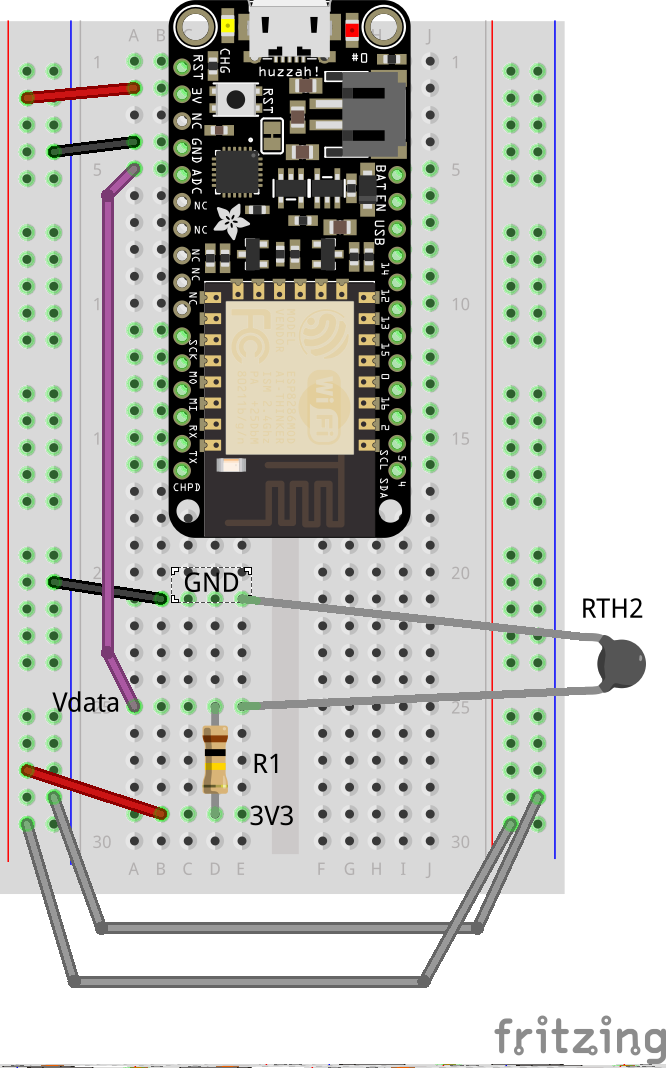
\includegraphics[width=\MFW]{Fritzing/feather_thermistor_bb.png}}{https://publicsensors.org/IntroSensors/Fritzing/feather_thermistor_bb.png}
		\caption[Thermistor circuit schematic]{An illustration of the layout for a circuit using a thermistor to measure temperature. 
			This schematic represents Configuration 2, in which the thermistor (here labeled \texttt{RTH2}) takes the place of resistor $R_2$ in the original voltage divider circuit.
			In Configuration 1, the thermistor would instead take the place of resistor $R_1$. 
			In the schematic, jumpers that are not needed but may be left in place if already present are indicated in gray.}
		\labfig{example_label}
	\end{center}
\end{marginfigure}

This figure can be referred to in the text with \verb|\reffig{example_label}| to produce a hyperlinked reference, as in \reffig{example_label}.

Note that the \verb|[-8cm]| in the marginfigure begin statement is a manual adjustment of the vertical position of the figure. 
This is for situations, which occur frequently, when the default placement of the figure (or, below, other margin content) is less than ideal.

Note also that figures and other margin content often require several \LaTeX compilations to acquire their final formatting, implement hyperlinks, \etc

\section{Notes, tables and margin content}
Several kinds of colored text boxes appear in the book, used to emphasize important points or provide background relevant to a specific idea or activity. 
As long as there are not too many of these special text boxes, they are both conspicuous while reading the text and easy to find later, if the reader remembers there was useful information somewhere but not where that was.
\subsection{Textboxes}
Textboxes are generally used for short sections of text that are integral parts of the text, but which are especially important for students to read and understand.
These often occur at the end of subsections, where readers whose patience is being tried by a long stream of detailed information may be tempted to skip them.

Textboxes appear in the default \verb|kaobox| color, currently light blue. 
They typically appear as their own separate paragraph, \eg,
  
\begin{verbatim}
\begin{kaobox}[frametitle=WiFi special powers]
	One of the best features of the ESP8266 is that it's
	 built-in WiFi can operate in both Access Point and 
	 Station mode simultaneously. 
	That is, you do not have to stop the connection in AP 
	mode to initiate a connection in station mode, or 
	\textit{vice versa}.
	
	Having these two types of connections at the same time
	 can be very useful.
	For example, if you move your microcontroller from 
	school to home, your classroom's Access Point is no 
	longer available.
	To connect to your home Access Point, you can log 
	directly onto your ESP8266 using its own AP mode SSID. 
	Using that connection, you can repeat the steps above, 
	with the name and password of your home Access Point, 
	to reconnect to the Internet.   
\end{kaobox}
\end{verbatim}

which results in

\begin{kaobox}[frametitle=WiFi special powers]
	One of the best features of the ESP8266 is that it's built-in WiFi can operate in both Access Point and Station mode simultaneously. 
	That is, you do not have to stop the connection in AP mode to initiate a connection in station mode, or \textit{vice versa}.
	
	Having these two types of connections at the same time can be very useful.
	For example, if you move your microcontroller from school to home, your classroom's Access Point is no longer available.
	To connect to your home Access Point, you can log directly onto your ESP8266 using its own AP mode SSID. 
	Using that connection, you can repeat the steps above, with the name and password of your home Access Point, to reconnect to the Internet.   
\end{kaobox}

\subsection{Sidenotes}
\emph{Sidenotes} are short snippets of text, functioning more as an aside than a ``plain'' textbox. 
Examples include concisely stating an idea complementary to those in the main text, a brief explanation or suggestion, or a relevant link.
Sidenotes are colored by the parameter \verb|\SNcolor|, currently light green. 

Sidenotes are produced by inclusions like
\begin{verbatim}
\sidenote[][*-4]{\begin{kaobox}[backgroundcolor=\SNcolor,
frametitlebackgroundcolor=\SNcolor,frametitle=Pass the
 word!]The best passwords are easy to remember and hard 
 to guess. One way to get good passwords is with a 
 utility called \texttt{apg}. \texttt{apg} generates 
 random passwords that are gibberish, so they're hard to 
 guess, but pronounceable, so they're easy to remember 
 by sound.  It is available for both \htmladdnormallink{Windows}
 {https://sourceforge.net/projects/apg-for-windows/} and 
 \htmladdnormallink{Macs and linux}{https://help.ubuntu.
 com/community/StrongPasswords}.\end{kaobox}}
\end{verbatim}
Sidenote inclusions are embedded within the sentence or paragraph to which they apply, and result in a in a footnote-style reference number
\sidenote[][*-4]{\begin{kaobox}[backgroundcolor=\SNcolor,frametitlebackgroundcolor=\SNcolor,frametitle=Pass the word!]The best passwords are easy to remember and hard to guess. One way to get good passwords is with a utility called \texttt{apg}. \texttt{apg} generates random passwords that are gibberish, so they're hard to guess, but pronounceable, so they're easy to remember by sound.  It is available for both \htmladdnormallink{Windows}{https://sourceforge.net/projects/apg-for-windows/} and \htmladdnormallink{Macs and linux}{https://help.ubuntu.com/community/StrongPasswords}.\end{kaobox}}
in addition to the sidenote.

Sidenotes sometimes have weak puns in their headers, the idea being that students will groan but nonetheless feel compelled to read them.

\subsection{Tables}
The primary use of tables in the current version of the book is in lists of materials.
Material lists that include inexpensive microcontrollers, sensors, connectors and other components are challenging in that the basic technologies, vendors and links to specific items change frequently.
The strategy for coping with this challenge adopted here is to have summary lists of materials, organized where possible by the subsections in which items are first required, in a highly condensed format at the beginning of each chapter.
This enables readers to anticipate which materials are required for given activities, and which activities are possible with a given set of materials.

These condensed tables include links to corresponding items in \refch{materials}, where a larger ``master'' table provides URLs to vendors or other information useful for acquiring components. 

It's to be expected that some of those URLs will become obsolete over relatively rapid timescales, but hopefully this information will still be a starting point for chasing down new components and vendors.

Materials lists currently have three columns: A section label, an item and a link to \refch{materials}.
An example materials table is
\begin{verbatim}
\begin{table}[h]
\caption[\refch{time_keeping} materials]{\textbf{Materials you'll need\dots} 

See Table \ref{tab:materials} for additional information.}
\labtab{materials_time_keeping}
\begin{center}
\raggedright
%\begin{tabular}{ c c c c } 
\begin{tabular}{ c r c}
\hline
Sections & item & link \\
\hline
\multirow{2}{4em}{\refsec{set_read_time}} 
& breadboard & \ref{mat:bb} \\
& ESP8266 ``Feather'' & \ref{mat:mc} \\
& micro-USB cable & \ref{mat:usb_cbl} \\
%		\hline
%		\multirow{3}{4em}{\vrefsec{circuits}}  
& male-male jumpers & \ref{mat:jmp_mm} \\ 
& pliers & \ref{mat:plr} \\ 
& DS3231 RTC & \ref{mat:RTC} \\ 
\hline
\end{tabular}

\end{center}\end{table}
\end{verbatim}
which produces 
\begin{table}[h]
	\caption[\refch{time_keeping} materials]{\textbf{Materials you'll need\dots} 
		
		See Table \ref{tab:materials} for additional information.}
	\labtab{materials_time_keeping}
	\begin{center}
		\raggedright
		%\begin{tabular}{ c c c c } 
		\begin{tabular}{ c r c}
			\hline
			Sections & item & link \\
			\hline
			\multirow{2}{4em}{\refsec{set_read_time}} 
			& breadboard & \ref{mat:bb} \\
			& ESP8266 ``Feather'' & \ref{mat:mc} \\
			& micro-USB cable & \ref{mat:usb_cbl} \\
			%		\hline
			%		\multirow{3}{4em}{\vrefsec{circuits}}  
			& male-male jumpers & \ref{mat:jmp_mm} \\ 
			& pliers & \ref{mat:plr} \\ 
			& DS3231 RTC & \ref{mat:RTC} \\ 
			\hline
		\end{tabular}
		
\end{center}\end{table}



\section{Milestones}
\begin{enumerate}
	\item Milestones document accomplished tasks or functioning hard- and software that: (a) enables instructors to assign credit for hands-on activities; and, (b) indicates to instructors and students competence in a given topic and readiness to proceed to subsequent topics.
	\item Milestones appear at relevant places in the text, typically immediately following the How-To Guide explaining how to accomplish the task.
	\item Milestones are reprinted together in \refch{milestones}. This is to make it easier to select among and modify the Milestones for a given classroom situation.
	\item Milestones descriptions should be short, and the required activities should be specific.
	\item Experience suggests that more, smaller Milestones are often more palatable to students than fewer, more complicated Milestones.
	\item Milestones are written in the document \texttt{Milestones.tex} in the \texttt{Chapters subdirectory}.
	\item The \LaTeX format for a Milestone is	
\color{blue}
\begin{verbatim}
%<*mlst:ex>
\begin{kaobox}[backgroundcolor=\MScolor,frametitlebackgroundcolor=\MScolor,
    frametitle=Milestones Example Title]
	\begin{itemize}
	\item [$\Box$] This is an example of a Milestone.\space 
	The specific goals are to demonstrate: (a) try it; and, 
	(b) be satisfied with the result. \,
	After you write a Milestone you like, complete the assignment by uploading a screenshot or 
	the \LaTeX version to receive credit.
\end{itemize}
\end{kaobox}
%</mlst:ex>
\end{verbatim}
\color{black}
	\item Milestones are invoked with the command
\color{blue}
\begin{verbatim}
	\loadMilestone{mlst:ex} % load milestone with tags id: mlst:ex}
\end{verbatim}	
\color{black}
	\item The result in this example is 
\begin{kaobox}[backgroundcolor=\MScolor,frametitlebackgroundcolor=\MScolor,
	frametitle=Milestones Example Title]
	\begin{itemize}
		\item [$\Box$] This is an example of a Milestone.\space 
		The specific goals are to demonstrate: (a) try writing one; and, 
		(b) be satisfied with the result. \,
		After you write a Milestone you like, complete the assignment by uploading a screenshot or 
		the \LaTeX version to receive credit.
	\end{itemize}
\end{kaobox}
\end{enumerate}
%\section{Text formatting}

\section{Scripting commands and codes}
\begin{enumerate}
	\item \textbf{Code listing in PDF LaTeX-generated PDF files (and probably many other PDF files) have an inherent problem that strings of space characters are absorbed into a unified white space. 
	This means that character-specific indentation is lost. 
	For this reason, all codes used in the book that are too long to quickly type directly into a \texttt{REPL} session should be posted and linked at a publicly available URL.}
	\item Short commands to be entered into a terminal window, such as those to invoke and use \mpfshell, are displayed using the \texttt{lstlisting} environment, e.g.
\begin{verbatim}
\begin{lstlisting}[language=bash]
pip3 install --upgrade --user mpfshell
\end{lstlisting}
\end{verbatim}
	which results in 
\begin{lstlisting}[language=bash]
pip3 install --upgrade --user mpfshell
\end{lstlisting}
Note that indentation in the \texttt{lstlisting} environment is reflected in the PDF, so it should not be included in the listing even if in an indented part of the text.
	\item Short Python commands are displayed using the \texttt{lstlisting} environment with language set to ``Python'', e.g.
\begin{verbatim}
\begin{lstlisting}[language=Python]
import network
ap = network.WLAN(network.AP_IF)
ap.config("essid")
\end{lstlisting}
\end{verbatim}
which results in
\begin{lstlisting}[language=Python]
import network
ap = network.WLAN(network.AP_IF)
ap.config("essid")
\end{lstlisting}
	\item Complete Python scripts and snippets of code too long to quickly type into a \texttt{REPL} session are saved in a separate file in the \texttt{Codes} subdirectory.  	
	These are inserted into the text with a command like
	\begin{verbatim}
	\lstinputlisting[language=Python,label=ButtonInterrupt,
	caption={\texttt{button\textunderscore interrupt.py}: 
	A Micropython script to toggle the state of GPIO 2 when 
	GPIO 0 changes state.}]{Codes/button_interrupt.py}
	\end{verbatim}
	A script inserted using this syntax will appear in the \texttt{Listings}, a hyperlinked table of contents for codes analogous to the \texttt{List of Tables} and \texttt{List of Figures} at the beginning of the book.
	
	\item In the example above, the script name has a ``\textunderscore'', which must be referred to using \verb|\textunderscore| in the caption. Otherwise a typesetting error will be triggered. 
	
	This may be a reason to avoid using underscores in script names, which are otherwise often useful.
	\item Complete Python scripts should be tagged with a hyperlink to a public URL where an updated version of the code is available to readers.
\end{enumerate}


\section{ToDo items}
\begin{enumerate}
	\item ToDo items should be high priority items, temporarily flagged for rapid resolution. 
	\item ToDo items appear as bright orange margin notes. They do not appear in the Table of Contents, but are easy to spot in the sidebar of most PDF viewers.
	\item ToDo items must indicate their author and creation date.
	\item ToDo items are written in the form
\begin{verbatim}
\todo{This is an example of a ToDo item. DG 1/4/20}
\end{verbatim}
	\item This results in a ToDo flag that looks like:
\todo{This is an example of a ToDo item. DG 1/4/20}
	\item See --- they're ugly! Please don't leave them in place more than a very short time. 
	\item Editors may comment out lingering ToDo items. They can still be found by searching in the \texttt{tex file.}
\end{enumerate}
%\section{Text formatting}


%provide you with the necessary skills and experience to design, build and use instruments to measure environmental conditions. 
%The ``brain'' of these instruments is a \emph{microcontroller}.
%A microcontroller is a device with a processing unit that can run codes and other instructions, and external connections (called \emph{pins}) to transmit electrical inputs and outputs. 
%The microcontroller is what enables your instrument to receive information from sensors, monitor and regulate its power supply, and communicate to receive instructions and telemeter data. 
%Learning to communicate with and control a microcontroller is the first step in building and using environmental sensors. 
%
%\begin{margintable}[2cm]
%	\caption[\refch{connect} materials]{\textbf{Materials you'll need\dots} 
%		
%		See Table \ref{tab:materials} for additional information.}
%	\labtab{materials_connections}
%	\raggedright
%	%\begin{tabular}{ c c c c }
%	\begin{tabular}{ c r c}
%		\hline
%		Sections & item & link \\
%		\hline
%		\multirow{3}{4em}{\refsec{connections}} 
%		& breadboard & \ref{mat:bb} \\
%		& ESP8266 ``Feather'' & \ref{mat:mc} \\
%		& micro-USB cable & \ref{mat:usb_cbl} \\
%		\hline
%		\multirow{1}{4em}{\refsec{WiFi_connect}}  
%		& WiFi router & \ref{mat:router} \\ 
%		\hline
%	\end{tabular}
%\end{margintable}
%
%There are many types of microprocessors, which vary by overall size, power requirements, capabilities to input and output different kinds of electrical signals, onboard communication hardware like WiFi or USB, and the types of code or instructions they accept. 
%%
%This textbook focuses on microprocessors that use instructions written in \htmladdnormallink{MicroPython}{https://micropython.org/}, a subset of the \htmladdnormallink{Python}{https://www.python.org} programming language.
%MicroPython is a recent invention, and a great improvement for learning about, building and using environmental sensors.
%Because MicroPython-based microcontrollers are automatically interactive
%\sidenote[][*4.5]{Like Python, MicroPython runs in an interactive session. 
%	This session goes by the  technical-sounding name \textbf{REPL}, which stands for ``Read-Evaluate-Print-Loop''.
%	%	, or \emph{REPL}. 
%	Despite this name, REPL is a very intuitive interface. 
%	REPL simply means that, in a MicroPython (or Python) session, you type commands, which are then executed, and the results are displayed.
%}
%, they are good platforms to develop and debug codes to collect data from environmental sensors.  
%
%Python itself is a powerful and easy to learn language for scientific computing on desktops and laptops. 
%If you already know some Python, you can apply that knowledge to working with MicroPython-based microcontrollers. 
%If you're new to Python, then by learning MicroPython you will simultaneously learn how to use Python for many other tasks. 
%%In fact, m
%Many of the exercises in this book combine acquiring data from sensors using a microcontroller, and analyzing or plotting those data on a computer, using the same Python coding language.
%
%\marginnote[1cm]{Note that Python is currently undergoing a transition, from an older version (Python 2.7) to newer Python 3 versions. 
%	These are mostly similar, but differ in some details such as the syntax of print commands. Because MicroPython is based on Python 3, and because older versions of Python will soon no longer be supported, the codes and instructions in this book will use Python 3.}
%%In most cases, Python 2.7 users will need to make only minor adjustments. 
%
%
%%\section{Meet your microcontroller}
%%\labsec{microcontrollers}
%
%\subsubsection{Adafruit's Feather HUZZAH ESP8266 microcontroller}
%
%
%For examples in this book, we will use Adafruit's Feather HUZZAH ESP8266 microcontroller. 
%It is small, has built-in WiFi, uses relatively little power, and is low cost for its capabilities. 
%The core ESP8266 microcontroller was originally intended to be placed in ``smart'' lightbulbs.\sidenote[][*+3]{See \htmladdnormallink{Tinnkerman's light bulb hacks}{https://tinkerman.cat/post/yet-another-wifi-light-bulb/} for some fun examples in which the ESP8266 microcontroller is reprogrammed in place within a smart light bulb.}
%Very large scale production for this purpose has made this microcontroller inexpensive, which also makes it a good choice for putting in sensors in often-harsh environments.
%
%Note that the exercises in this book can be successfully completed using other microcontrollers. 
%We focus here on the Feather ESP8266 because it's one of the microcontrollers officially supported by \htmladdnormallink{MicroPython}{https://http://micropython.org/}, because Adafruit provides good documentation and support for it, and because it's likely to be available for some time into the future.
%The other officially supported microcontroller, Adafruit's HUZZAH ESP8266 Breakout Board, is slightly smaller and cheaper, but requires a special cable for communications rather than a generic microUSB cable.
%Other manufacturers also make microcontroller boards based on the ESP8266. 
%Many of these will work in essentially the same way for exercises in this book. 
%Boards using other processors also can work. 
%These alternative microcontrollers may require modifying details in the MicroPython codes, such as the numbers for electrical inputs and outputs. 
%The \htmladdnormallink{MicroPython}{https://http://micropython.org/} website is the best reference if you are considering using alternative microprocessor boards for the activities in this book.
%
%\begin{marginfigure}[8cm]
%	\begin{center}
%		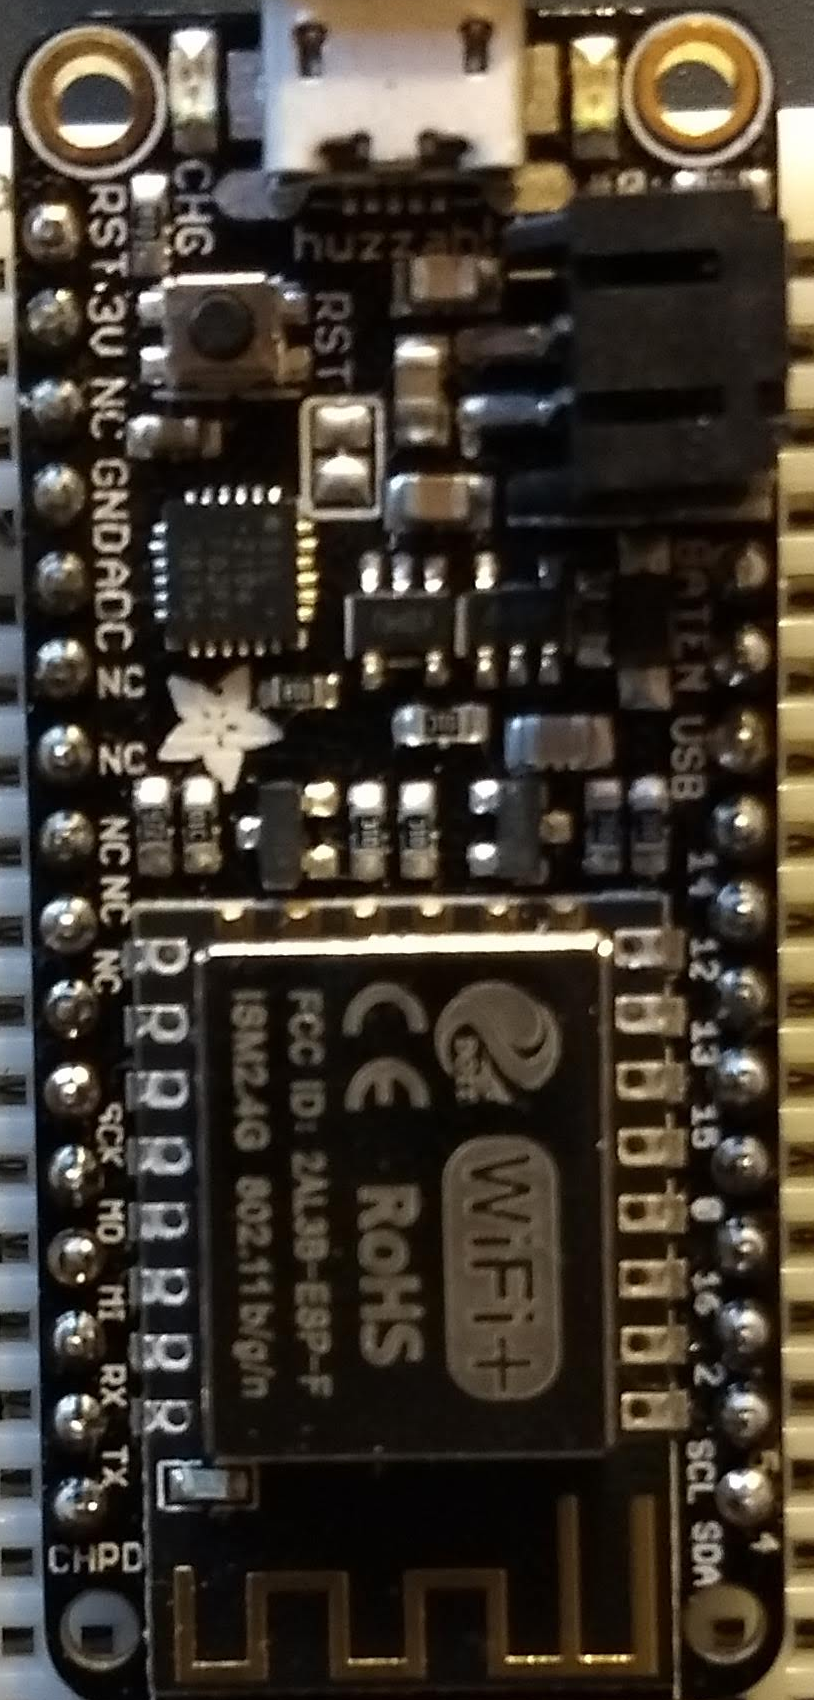
\includegraphics[height=6cm]{Images/ESP8266feather_top.png}
%		\caption[ESP8266 feather microcontroller]{A ESP8266 Feather microcontroller.}
%		\labfig{margin_esp8266}
%	\end{center}
%\end{marginfigure}
%
%A close-up view of the ESP8266 Feather (\reffig{margin_esp8266}) shows the key features we will use to create functional environmental sensors.
%\marginnote[-0cm]{
%	The documents \htmladdnormallink{adafruit-feather-huzzah-esp8266.pdf}{https://cdn-learn.adafruit.com/downloads/pdf/adafruit-feather-huzzah-esp8266.pdf} and \htmladdnormallink{adafruit-huzzah-esp8266-breakout.pdf}{https://cdn-learn.adafruit.com/downloads/pdf/adafruit-huzzah-esp8266-breakout.pdf} are the best overall resources for information about the Adafruit Huzzah Feather and Breakout versions of the ESP8266 microcontroller. 
%	Please download the document for your microcontroller for future reference about specifications, pin definitions, voltage tolerances, \etc
%}
%The core microcontroller is the rectangular component near the bottom.
%The zigzag line below it is a built-in WiFi antenna. 
%At the top is a connector for a microUSB cable, used to communicate with the Feather. 
%Plugging a USB cable into this connector and into your computer automatically supplies power to the microcontroller. 
%It also automatically supplies a connection for communicating with the microcontroller.% -- see \refsec{usb_connect} for instructions on how to use USB to communicate with your microcontroller.
%
%Below and to the left of the USB connector is a button, labelled ``\texttt{RST}''. 
%This is a reset button, used occasionally to halt a run-away code or reboot a malfunctioning microcontroller (normally we will do this via software, so we rarely need to use the \texttt{RST} button).
%At the four corners are holes for mounting screws. 
%Along the right and left edges are soldered ``pins'', %which are spaced to fit into a breadboard, and 
%which have different capabilities to transmit electrical signals to and from the microcontroller. 
%These pins have labels alongside (sometimes a little above or below) that identify the pin, so it can be referred to in MicroPython codes. 
%We will explain how to use these pins in \refch{first_exercises}. 
%
%
%%\begin{marginfigure}[0cm]
%%	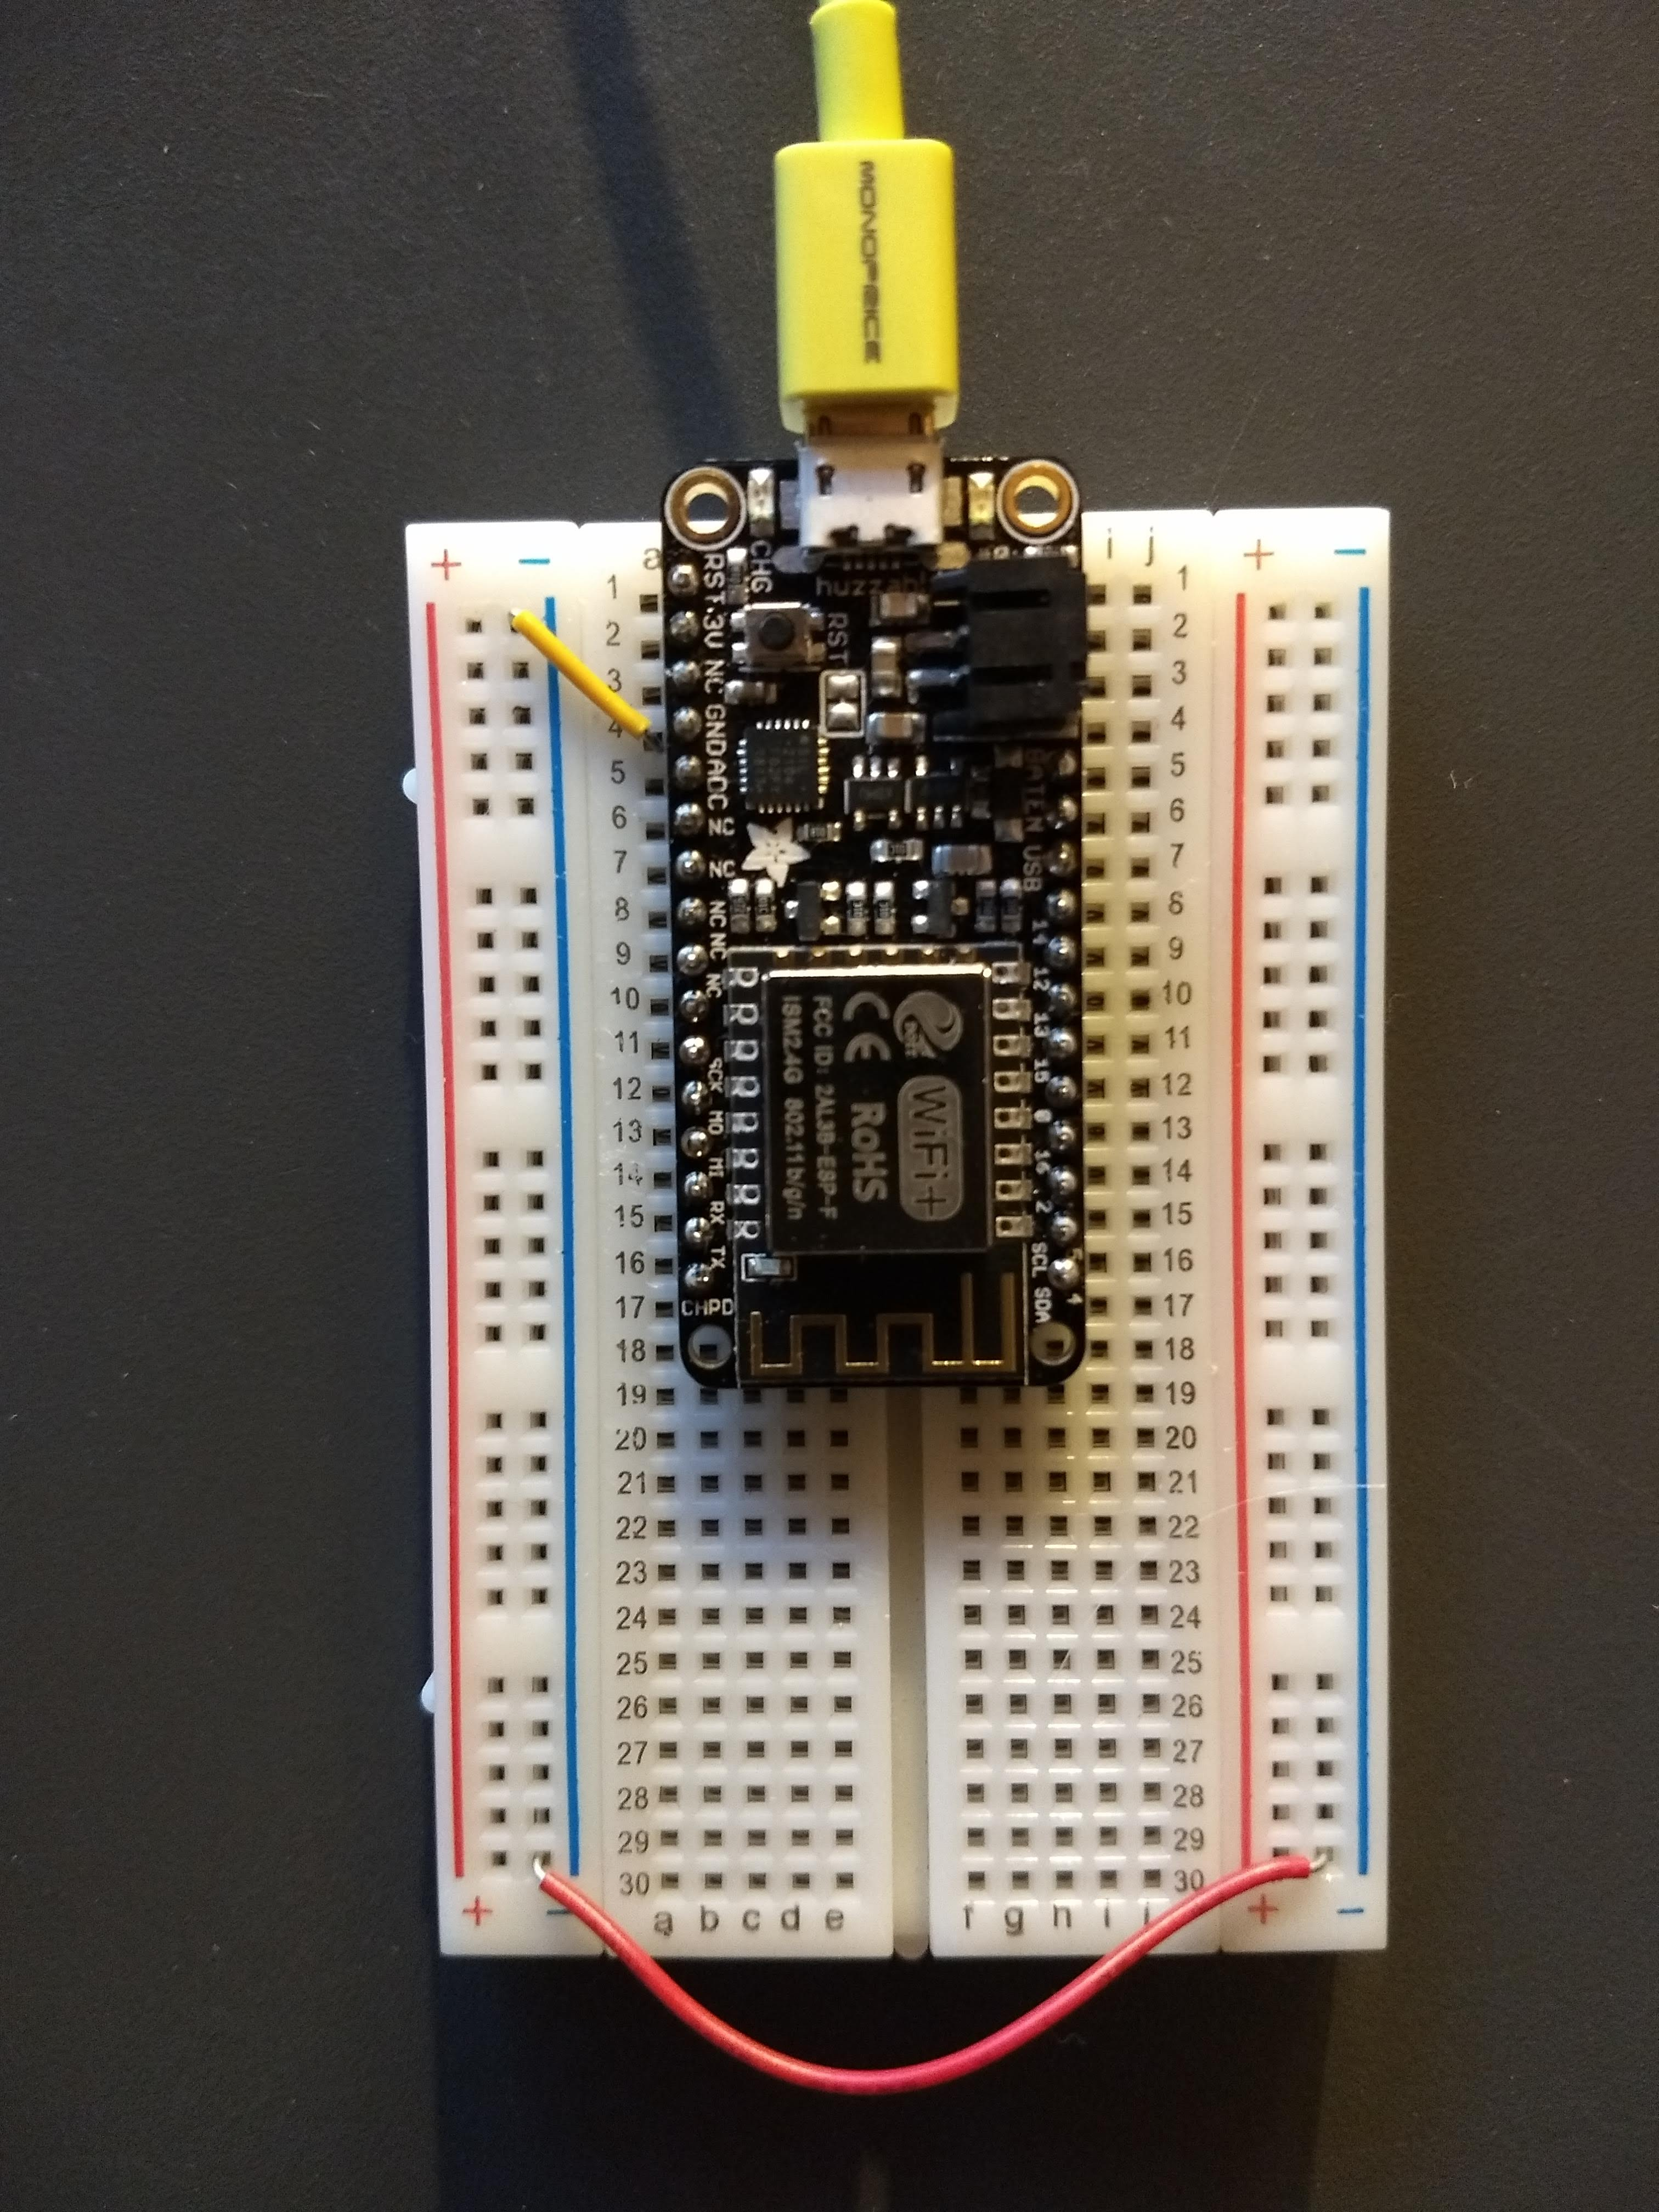
\includegraphics{Images/breadboard_ESP8266feather.jpg}
%%	\caption[ESP8266 feather microcontroller on breadboard]{Breadboard with ESP8266 feather.}
%%	\labfig{margin_breadboard_esp8266}
%%\end{marginfigure}
%
%%%
%%%\begin{lstlisting}
%%%	\begin{marginfigure}
%%%		\includegraphics{Images/IMG_20181205_082817686.jpg}
%%%		\caption[ESP8266 feather microcontroller on breadboard, too]{Breadboard with ESP8266 feather, again.}
%%%		\labfig{esp8266brd}
%%%	\end{marginfigure}
%%%\end{lstlisting}
%%
%
%\section{Establishing communications}
%\labsec{connections}
%
%Our starting point for building and using environmental instruments is learning how to communicate with microcontrollers from your desktop or laptop computer. 
%The ESP8266 Feather (and many other microcontrollers) have two primary modes of communication: USB and WiFi. 
%Some microcontrollers have additional communication modes, such as BlueTooth, LoRa or other wireless protocols.
%However, USB and WiFi are the most common, standardized and useful communication modes for microcontrollers, so in this book we focus on these two modes. 
%
%In general, either USB or WiFi mode alone can be sufficient for building and using environmental sensors.
%However, it is often very helpful to have both options. 
%For example, WiFi connections can be very useful when working with microcontrollers in environmental sensing instruments, which are often deployed inside waterproof housings that make it impossible to connect a cable. 
%On the other hand, when generating and debugging codes to run these instruments, it is frequently necessary to reboot the microcontroller. 
%This breaks the WiFi connection, so that the REPL session (and usually the WiFi connection itself) must be re-initiated. 
%In this case a USB connection, which remains active through the reboot, may be more convenient.
%
%To work efficiently and effectively with microcontrollers, we require two essential communication functions: 
%\begin{enumerate}
%	\item We need to be able to issue commands and see output during a REPL session; and, 
%	\item We need to transfer files, such as MicroPython codes and environmental data, on and off the microcontroller's flash memory.
%\end{enumerate} 
%Both these functions can be accomplished using either USB or WiFi. 
%
%Below, we describe two alternative approaches for communicating with  ESP8266 microcontrollers running MicroPython. Both are free, and can be implemented on most desktop and laptop computers. 
%\begin{itemize}
%	\item Google's Chrome browser, with extensions enabling communications via USB and WiFi. 
%	\item \mpfshell, a command line utility (that is, a small Python script that works within a simple terminal window).
%\end{itemize}
%Of the two, the Chrome browser approach has the advantages that it is very easy to install on most computers, and it looks and acts very much the same across Windows, Mac OS, Chromebooks and linux computers. 
%However, the Chrome interface is slower and in some ways less capable. 
%Also, the only browser-based method currently available to transfer files to/from the microcontroller is through WiFi (using WebREPL, described below). 
%
%\mpfshell can both support a REPL session and transfer files, over either USB or WiFi. 
%The \mpfshell approach requires that Python be installed on your computer, if it is not already 
%(Mac OS and linux machines have Python pre-installed, but many Windows users must install it, and \mpfshell is not available for Chromebooks). 
%While this installation may require some extra effort, working with microcontrollers through \mpfshell is so much more effective that we recommend you take this approach whenever possible.
%
%
%%\marginnote[0cm]{
%\begin{kaobox}[frametitle=As you get started \dots]
%	One of the challenges in working with microcontrollers is that the first step -- establishing communications -- is often the fussiest part of the entire process. 
%	That is because, while the microcontrollers are relatively standardized, the computers we use to communicate with them have highly variable and frequently changing hardware and software. 
%	These variations may results in differences in drivers, ports and communications software between. 
%	\emph{It's important to approach this first step patiently and systematically, and to be prepared to ask for help from experienced people in person or online.}
%	In addition to the instructions in this chapter, tutorials for setting up and troubleshooting USB and WiFi connections can be found at the \htmladdnormallink{MicroPython}{https://micropython.org/} website and many other resources online.
%\end{kaobox}
%%}
%
%
%\section{Connecting to your microcontroller via USB}
%We will first take you through the steps necessary to connect to your microcontroller using USB. In \refsec{WiFi_connect}, we will use this USB connection to set up your microcontroller for WiFi connections.
%
%\subsection{Installing the driver for USB connections}
%If your laptop runs Windows, OS X (Mac) or Chrome, you will need to install a driver to enable your computer to connect with serial USB converter on your ESP8266 Feather microcontroller (this is not needed on linux machines). 
%The driver is available at \htmladdnormallink{this link}{https://www.silabs.com/products/mcu/Pages/USBtoUARTBridgeVCPDrivers.aspx}. 
%
%Computers with older operating systems may require an older version of the driver. 
%If you install the newest one and still cannot connect to the microcontroller, try installing the next older one. 
%Note that you must \emph{uninstall} the existing driver version \emph{before} installing a different version. 
%Instructions are included in the downloaded package files, and on the download website.
%
%\subsection{USB connections via Chrome}
%If you will use Chrome for your microcontroller work, you can install it from Google's \htmladdnormallink{download page}{https://www.google.com/chrome/}. 
%For USB connections, you need to install an extension called \textbf{BeagleTerm}. 
%From a Chrome window, navigate to  \htmladdnormallink{this link}{https://chrome.google.com/webstore/detail/beagle-term/gkdofhllgfohlddimiiildbgoggdpoea?hl=en}, and use the button at the upper right to install it. 
%BeagleTerm will now appear in your list of \htmladdnormallink{Apps}{chrome://apps/}.
%
%\begin{marginfigure}[-4cm]
%	\begin{center}
%		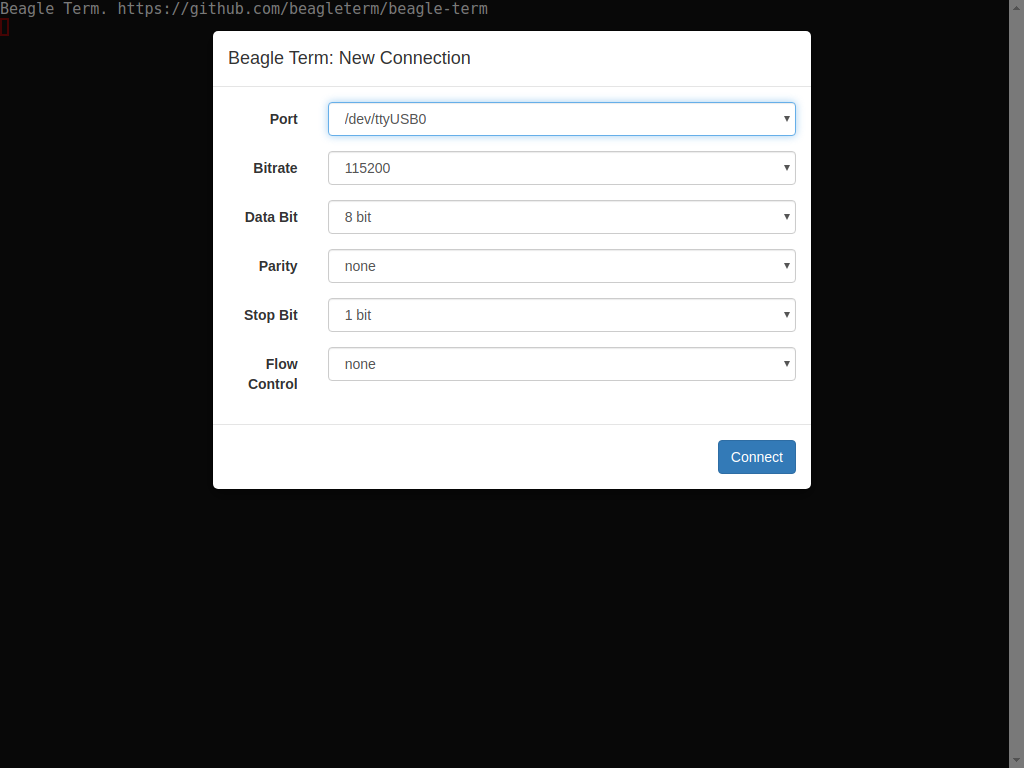
\includegraphics[width=\MFW]{Images/BeagleTermConnect.png}
%		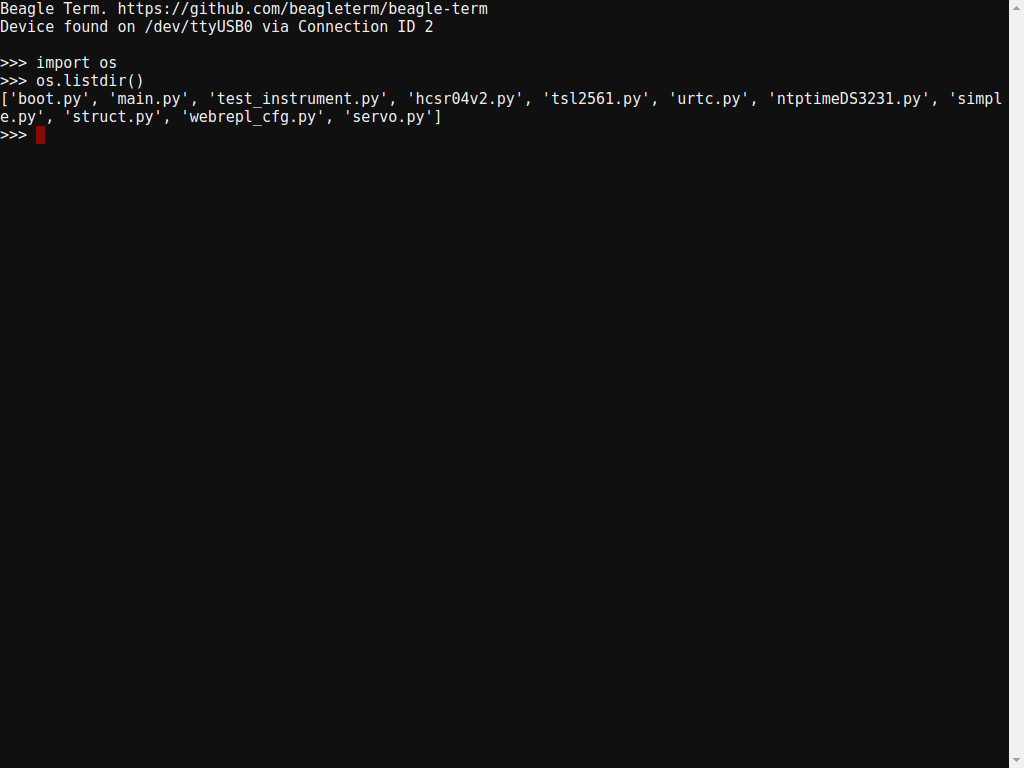
\includegraphics[width=\MFW]{Images/BeagleTerm.png}
%		%		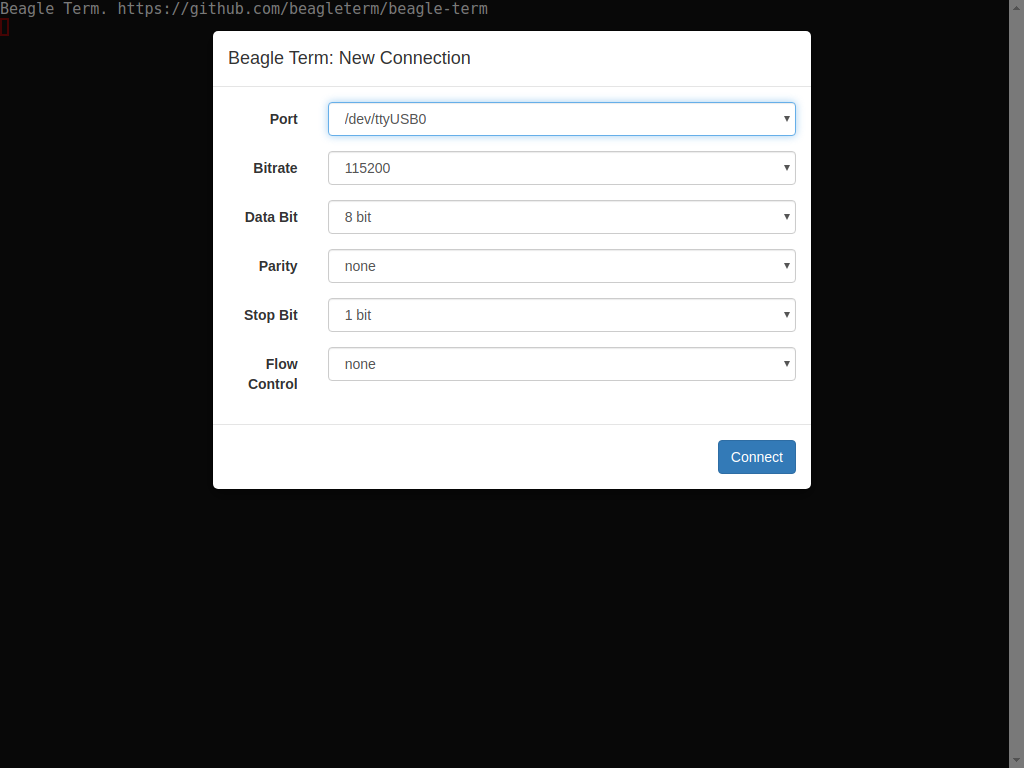
\includegraphics[width=5cm]{Images/BeagleTermConnect.png}
%		\caption[Connection via BeagleTerm.]{BeagleTerm browser windows. Upper screenshot: The connection prompt with settings. Most of these default into the correct values. The Com port setting, in this case \texttt{ttyUSB0}, is the most likely one you may need to change. Lower screenshot: After connecting, press \texttt{return} on your keyboard to start a REPL session.}
%		\labfig{BeagleTermConnect}
%	\end{center}
%\end{marginfigure}
%
%To connect to your microcontroller via BeagleTerm (\reffig{BeagleTermConnect}):
%\begin{enumerate}
%	\item Plug a USB cable into your computer and your microcontroller (before you launch BeagleTerm). 
%	\item Launch the BeagleTerm app. 
%	
%	Usually the default parameters are correct, if the USB cable is already connected to both the computer and microcontroller when the app launches.
%	\item Click ``Connect'' and press ``Enter'' a couple times on your keyboard. 
%	
%	You should now see a ``\verb|>>>|'' Python prompt, meaning you are connected and ready to work with your microcontroller.
%\end{enumerate}
%If this does not work, the culprit is usually the ``Com port'' setting.
%Use the menu to try the available ports until you find the right one.
%
%%Note that there is currently no way (other than copying and pasting) to transfer files between your computer and microcontroller via a USB cable. 
%
%\subsection{USB connections via \mpfshell}
%\mpfshell is a Python-based file explorer and serial communications package. 
%For communication with ESP8266-based microcontrollers, we have found \mpfshell to be the most convenient utility, because it includes both key communications functions.
%Users can rapidly switch between interactive REPL sessions and file transfers, with a few keystrokes.
%\mpfshell also works over both USB and WiFi.
%
%\subsubsection{To install \mpfshell:}
%
%Instructions for installing and using \mpfshell are at \htmladdnormallink{this link}{https://github.com/wendlers/mpfshell}. 
%\mpfshell requires that Python be installed on your computer, preferably the most recent version (currently 3.5.9). 
%Machines running OS X or linux have Python pre-installed. 
%See links at \htmladdnormallink{Python}{https://www.python.org/downloads/windows/} and \htmladdnormallink{mpfshell}{https://gist.github.com/hardye/657385210c5d613e69cb5ba95e8c57a7} for instructions on installing Python and \mpfshell on Windows machines.
%
%\marginnote[-4cm]{
%	\mpfshell generally works when installed and used within a Python IDE such as \htmladdnormallink{Enthought Canopy}{https://assets.enthought.com/downloads/}. 
%	Python IDEs can have advantages in generating and debugging code. 
%	However, in some cases, we have found that functions such as copying and pasting text in REPL sessions have been more limited within an IDE session than when running Python within a simple terminal. 
%	When possible, therefore, we recommend running \mpfshell from a simple terminal, even if you like to edit code from within an IDE. 
%}
%With Python3 installed, the \texttt{pip3} utility makes it straightforward to install \mpfshell and a few other Python packages it requires:
%\begin{enumerate}
%	\item \textbf{Open a terminal window.}
%	\item \textbf{Install the latest version of \mpfshell and the packages it requires.}
%	
%	Use the command\sidenote[][*+0]{In this book, we will use this format to indicate code to be entered typed into a REPL session on your microcontroller, or to be put into a file to be run on your microcontroller or laptop.}
%	\begin{lstlisting}[language=bash]
%	pip3 install --upgrade --user mpfshell
%	\end{lstlisting}
%	Note that your computer needs to be connected to the Internet to access the necessary software repositories.
%\end{enumerate}
%
%\subsubsection{To connect to your microcontroller via \mpfshell:}
%
%\begin{enumerate}
%	\item \textbf{Plug a USB cable into your computer and your microcontroller} (before you launch \mpfshell). 
%	\item \textbf{Determine the correct port number.}
%	
%	On Mac OS and linux computers, issue the command
%	\begin{lstlisting}[language=bash]
%	ls -lht | head -n 30
%	\end{lstlisting}
%	The output from this command is a list of the most recent ``devices'' attached to the computer. If you recently plugged in your microcontroller, its port name should be something like \texttt{ttyUSB0} at or near the top of this list.	
%	\todo{Need instructions how to determine the com port on Windows, analogous to  on linux, Macs?}
%	\item \textbf{Launch \mpfshell}: 
%	\todo{Is being a member of the dialout group necessary to make this work without sudo?}
%	\begin{lstlisting}[language=bash]
%	mpfshell
%	\end{lstlisting}
%	You should now see a prompt like ``\verb|mpfs [/]>|''. This prompt means you are in ``file transfer mode''. 
%	\item \textbf{Open a connection to the microcontroller, using the port name from Step 2}:
%	\begin{lstlisting}[language=bash]
%	open ttyUSB0
%	\end{lstlisting}
%	You should get a response like ``\texttt{Connected to esp8266}''.
%	\item You can now use simple commands to: \begin{itemize}
%		\item \textbf{List the files} on your microcontroller (\texttt{ls}) or in your laptop's directory (\texttt{lls}); 
%		\item \textbf{Upload a file} from your laptop to your microcontroller (e.g., \texttt{put blah.py}); or,
%		\item \textbf{Download a file} from your microcontroller to your laptop (e.g., \texttt{get blah.py}).
%	\end{itemize} 
%	Many other commands are available in \mpfshell.
%	You can learn about them by executing %\texttt{help}
%	\begin{lstlisting}[language=bash]
%	help
%	\end{lstlisting}
%	or looking on the \htmladdnormallink{mpfshell github site}{https://github.com/wendlers/mpfshell}.
%	\item \textbf{Switch into the REPL session with the command:}
%	\begin{lstlisting}[language=bash]
%	repl
%	\end{lstlisting}
%	You should now see a ``\verb|>>>|'' Python prompt, meaning you are connected and ready to work with your microcontroller.
%	
%	\item \textbf{Switch back into file transfer mode:}
%	When you switch into \texttt{REPL}, \mpfshell gives you a message just above the first Python prompt similar to
%	\begin{lstlisting}[language=bash]
%	*** Exit REPL with Ctrl+] ***
%	\end{lstlisting}
%	% \verb|*** Exit REPL with Ctrl+] ***|. 
%	This tells you the command to switch out of the REPL session and back into file transfer mode (in this case, pressing the \verb|Ctrl| and \verb|]| keys on your keyboard simultaneously).
%	
%	You can switch back and forth between REPL and file transfer mode as many times as you want, as you edit your code, upload and execute it on your microcontroller, download data, \etc
%	
%\end{enumerate}
%\loadMilestone{mlst:ov} % load milestone with tags id: mlst:ov}
%\loadMilestone{mlst:01} % load milestone with tags id: mlst:01
%
%
%
%\section{Connecting to your microcontroller via WiFi}
%\labsec{WiFi_connect}
%Our first use of the USB REPL connection will be to set up connections by WiFi. 
%You will then have both options as you work through other activities in this book.
%
%\subsection{WiFi Access Points and Stations}
%First, a bit of background: Your ESP8266 has two modes for its wifi connections: \emph{Access Point} mode, and \emph{Station} mode. 
%In Access Point mode, your microcontroller accepts logins from other machines, such as your laptop. 
%This mode is useful, among other reasons, because when you set its name and password they do not change until you explicitly change them. 
%This means that when you change locations or work in areas lacking Internet access, you can still connect with your microcontroller.  
%In Station Mode, your microcontroller logs onto an existing Access Point, e.g. your home or classroom router.
%This mode is useful, among other reasons, because it enables your microcontroller to transmit data to and from the Internet. 
%\begin{itemize}
%	\item [(A)] \textbf{Access Point mode}
%	
%	Your ESP8266 is by default configured as an \emph{Access Point}, or \texttt{AP}. 
%	That means it serves as host for WiFi connections, like a router does: you can log directly onto your ESP8266’s AP via your computer’s wifi.
%	
%	To do this, you need to know what is its \texttt{SSID} (the name of the \texttt{AP} station, which appears as an entry in your computer's WiFi settings). 
%	By default, MicroPython sets your SSID to be of the format
%	\begin{lstlisting}[language=bash]
%	MicroPython-xxx
%	\end{lstlisting}
%	where \verb|xxx| is different for every individual ESP8266. 
%	
%	If there are many microcontrollers around, how do you know which is yours? 
%	Connect to your microcontroller over your USB cable. 
%	You can now query the AP status as follows:
%	\begin{lstlisting}[language=Python]
%	import network
%	ap = network.WLAN(network.AP_IF)
%	ap.config("essid")
%	\end{lstlisting}
%	The output from this command is your microcontroller's SSID.
%	
%	When they come from the factory, all ESP8266’s running Micropython have similar SSIDs and the same password, “\texttt{micropythoN}” (note the capital ``N''). 
%	That means it's easy to accidentally login onto the wrong microcontroller.
%	Not good!
%	
%	You can reset the parameters of your microcontroller's \texttt{AP} with a command of the following form:
%	\begin{lstlisting}[language=Python]
%	ap.config(essid="dannyESP8266", authmode=network.AUTH_WPA_WPA2_PSK, password="dg_sEns0r")
%	ap.active(True)
%	\end{lstlisting}
%	Here, the \texttt{AP} is set to have \verb|dannyESP8266| as its SSID, to have \texttt{WPA/WPA2} encryption, and to have the password ``\verb|dg_sEns0r|''.
%	Then, the \texttt{active} parameter is set to \lstinline|True|, meaning the Access Point is turned on. 
%	
%	Try it with your microcontroller, with a SSID that you can easily recognize as your own, and a hard to guess password.
%	%, hopefully with a password that is harder to guess than I used in this example. 
%	The password must be at least 8 characters long. 
%	WRITE THE SSID AND PASSWORD DOWN AND PUT THEM SOMEWHERE SAFE. 
%	
%	Now you should be able to log on from your computer using the new SSID and password.
%	Try it, by opening your WiFi settings, selecting your microprocessor's AP, and entering the password. 
%	
%	After your computer successfully connects, you are ready to interact with your microcontroller over WiFi using WebREPL or \mpfshell as described below.
%	
%	Use 
%	\begin{lstlisting}[language=Python]
%	ap.active(False)
%	\end{lstlisting}
%	%when you're ready to turn the AP off.
%	if you decide you no longer want your microcontroller's Access Point to be available.
%	
%	\item [(B)] \textbf{Station mode}
%	
%	To connect your ESP8266 to the Internet, you need instead to configure it in \texttt{Station} mode. 
%	In this mode, your computer cannot log directly onto your ESP8266.
%	Instead, your ESP8266 can log onto another Access Point, such as the WiFi router available in your home or classroom.
%	Then your computer (or any other machine) logged onto that router can connect to your microcontroller.
%	
%	Let's suppose the WiFi router available in your workspace has the SSID ``\texttt{SchoolSSID}'' and the password ``\texttt{top secret!}''.
%	Here is the command sequence:
%	\begin{lstlisting}[language=Python]
%	import network # Not necessary if you already did it in (A) 
%	wlan = network.WLAN(network.STA_IF)
%	wlan.active(True)         # activate the interface
%	wlan.connect("SchoolSSID", "top secret!")
%	\end{lstlisting}
%	In this mode, the IP number of your microcontroller is assigned by the OTCnet router. 
%	To see what it is, use the command
%	\begin{lstlisting}[language=Python]
%	wlan.ifconfig()
%	\end{lstlisting}
%	The result will be a group of numbers enclosed in parentheses (a Python ``tuple'') similar to 
%	\begin{lstlisting}[language=Python]
%	("192.168.0.9","255.255.255.0","192.168.0.1","192.168.0.1")
%	\end{lstlisting}
%	In this output, the first entry is your ESP8266’s IP address (this is the one you care about). 
%	The others are the router’s network mask, gateway and DNS server addresses. 
%	
%	When your microcontroller and your computer are both successfully logged onto the same Access Point, you are ready to interact with your microcontroller over WiFi using WebREPL or \mpfshell as described below.
%	
%	Use 
%	\begin{lstlisting}[language=Python]
%	wlan.active(False)
%	\end{lstlisting}
%	%when you're ready to turn the AP off.
%	if you decide you no longer want your microcontroller to try to log onto this Access Point (e.g., if you have changed location).
%	\marginnote[-2cm]{	A foible of the ESP8266 is that it repeatedly puts out debugging messages if it fails to connect to an Access Point when Station mode is active.
%		This does not interfere with interpretation of commands you send to the microcontroller, but is visually distracting.
%		To stop this unhelpful output, set it to inactive with the command \texttt{wlan.active(False)}.	
%	}
%	%	\begin{lstlisting}[language=Python]
%	%	\end{lstlisting}
%	%}
%\end{itemize}
%
%%\marginnote[0cm]{
%\begin{kaobox}[frametitle=WiFi special powers]
%	One of the best features of the ESP8266 is that it's built-in WiFi can operate in both Access Point and Station mode simultaneously. 
%	That is, you do not have to stop the connection in AP mode to initiate a connection in station mode, or \textit{vice versa}.
%	
%	Having these two types of connections at the same time can be very useful.
%	For example, if you move your microcontroller from school to home, your classroom's Access Point is no longer available.
%	To connect to your home Access Point, you can log directly onto your ESP8266 using its own AP mode SSID. 
%	Using that connection, you can repeat the steps above, with the name and password of your home Access Point, to reconnect to the Internet.   
%\end{kaobox}
%%}
%
%\loadMilestone{mlst:01a} % load milestone with tags id: mlst:01a
%
%
%\subsection{WiFi connections using \texttt{WebREPL} in a browser}
%\texttt{WebREPL} is a way for you to use a browser window to log directly onto your microcontroller, when it has an active WiFi interface (either in Access Point or Station mode). 
%\begin{marginfigure}[6cm]
%	\begin{center}
%		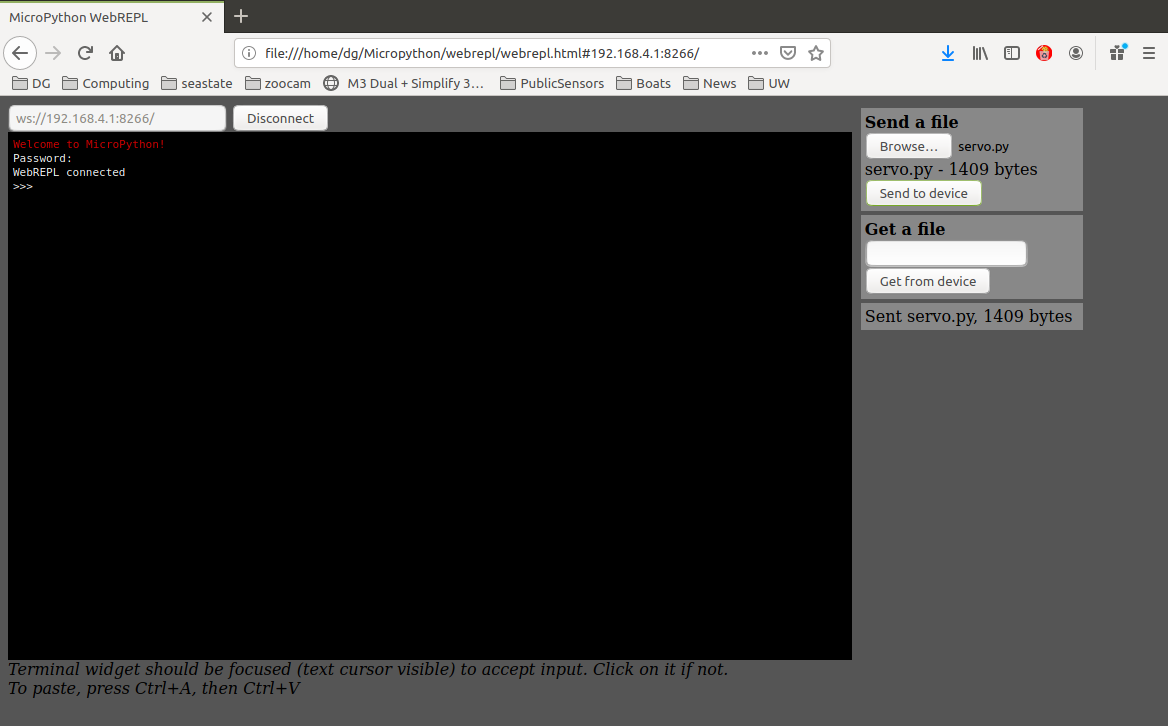
\includegraphics[width=5cm]{Images/WebREPLupload2.png}
%		\caption[A WebREPL session with upload.]{An active WebREPL session, showing the login prompt (main terminal frame) and a file upload (right side panel.}
%		\labfig{WebREPL_upload}
%	\end{center}
%\end{marginfigure}
%\texttt{WebREPL} can do both of the essential elements of communicating with microcontrollers, via a wireless connection:
%It provides access to REPL, and makes it very easy to upload and download files between your laptop and the ESP8266 (\reffig{WebREPL_upload}).
%
%%Note: Your microcontroller has to be connected via wifi for WebREPL to work, either with your laptop logged onto an Access Point created by the microcontroller, or with both your laptop and microcontroller logged onto another Access Point.
%
%WebREPL is a free download from this \htmladdnormallink{link}{https://github.com/micropython/webrepl}.
%An easy way to install the WebREPL archive on your machine is downloading the \htmladdnormallink{zipped package}{https://github.com/micropython/webrepl/archive/master.zip}.
%Some useful introductory information on using WebREPL is provided by Adafruit 
%\htmladdnormallink{here}{https://learn.adafruit.com/micropython-basics-esp8266-webrepl/access-webrepl},
%\htmladdnormallink{here}{https://learn.adafruit.com/micropython-basics-esp8266-webrepl/overview} and
%\htmladdnormallink{here}{https://learn.adafruit.com/micropython-basics-esp8266-webrepl/send-and-get-files}.
%%\begin{verbatim}
%%https://learn.adafruit.com/micropython-basics-esp8266-webrepl/access-webrepl
%%https://learn.adafruit.com/micropython-basics-esp8266-webrepl/overview
%%https://learn.adafruit.com/micropython-basics-esp8266-webrepl/send-and-get-files
%%\end{verbatim}
%
%\marginnote[-6cm]{Note that \texttt{WebREPL} is available to use online, without installing it. 
%	\emph{However, you will most likely want to have it actually installed directly on your computer.} 
%	That is because, unless you have multiple wireless connections available on your computer, you can’t use the online WebREPL when you connect directly to your ESP8266 as an Access Point.
%	You can, however, use the online \texttt{WebREPL} if your laptop and microcontroller are both logged onto another Access Point. 
%	We recommend installing \texttt{WebREPL} on your computer because in the upcoming activities you will likely have your microcontroller connected as a station and as an access point at various times.} 
%
%To launch WebREPL on your computer:
%\begin{itemize}
%	\item  Open the file \texttt{webrepl.html} in the \texttt{webrepl} directory (which you unzipped from the archive you downloaded from \texttt{github}). 
%	
%	WebREPL should work equally well in Chrome, Firefox, Chromium, Opera and other browsers. 
%	You should see a window like \reffig{WebREPL_upload} appear in your browser. 
%	
%	\item Enter the IP number in the text box at the upper left.
%	
%	%	Note that the IP number over which to connect is specified in the text box at the upper left.
%	If you are connected to your microcontroller's own Access Point (meaning its AP mode is active and your laptop is logged on) then the default value is correct -- you don't have to change anything.
%	
%	If you are using a router, you will likely need to change the IP number in this box to reflect the IP assigned by the router to your ESP8266. This is the first entry in the result of the \texttt{wlan.ifconfig()} command above.
%	
%	In either case, leave the port number the same (this is the part after the colon). 
%	
%	\item Click “Connect” and (after an additional prompt for your password) you should see the new connection reflected in a \verb|>>>| python prompt.
%	
%\end{itemize}
%%Summary: 1) Open webrepl.html in a browser; 2) Enter IP number in text box; 3) Click Connect \& enter password 
%
%%\marginnote[0cm]{
%\begin{kaobox}[frametitle=Making sure WebREPL is active on your microcontroller \dots]
%	WebREPL has two parts: One is the web page that you open on your laptop. The other is a Python script called \texttt{webrepl}that runs on your microcontroller, which must be activated for you to connect. 
%	
%	There are a couple of important details in making sure that WebREPL is activated on your microcontroller:
%	\begin{itemize}
%		\item The first time you want to connect via WebREPL, you need to initialize \texttt{itwebrepl} (set a password, \etc) by using your USB connection to issue the command
%		\begin{lstlisting}[language=Python]
%		import webrepl_setup
%		\end{lstlisting}
%		Three things then happen:
%		\begin{itemize}
%			\item The microcontroller will query you whether you want to enable \texttt{webrepl} (automatically start it each time the microcontroller reboots). Enter \texttt{E} to enable.
%			\item The microcontroller will prompt you for a password, which you need to enter twice. 
%			\item The microcontroller will ask whether to reboot, which is necessary to implement your new settings (Enter \texttt{y}, for yes).
%		\end{itemize}
%		When you have finished these three steps, \texttt{webrepl} will start by default with the password you set.
%		
%		\item If you are connected to your microcontroller via USB, sometimes \texttt{webrepl} does not run even if you set it to. In that case, you need to use your USB connection to execute the commands
%		\begin{lstlisting}[language=Python]
%		import webrepl
%		webrepl.start()
%		\end{lstlisting}
%		to manually start \texttt{webrepl}. Your microcontroller will then be available to connect via the WebREPL browser window.
%	\end{itemize}
%	
%	
%\end{kaobox}
%%}
%
%\subsubsection{Up- and downloading files over WiFi with \texttt{WebREPL}}
%\texttt{WebREPL} makes it easy to transfer files from your laptop to your microcontroller and \textit{vice versa}. 
%
%\textbf{To upload a file to your microcontroller (\reffig{WebREPL_upload}):}
%\begin{enumerate}
%	\item Click on the \texttt{Browse} button at the upper right of the \texttt{WebREPL} window,under the \texttt{Send a file} prompt. 
%	\item Navigate to and select the file you want to transfer (in this example, a file called \texttt{servo.py}).
%	\item Click the \texttt{Send to device} button. 
%	
%	The textbox at the bottom of the right side panel will now report the file sent and the number of bytes uploaded.
%\end{enumerate}
%
%\begin{marginfigure}[0cm]
%	\begin{center}
%		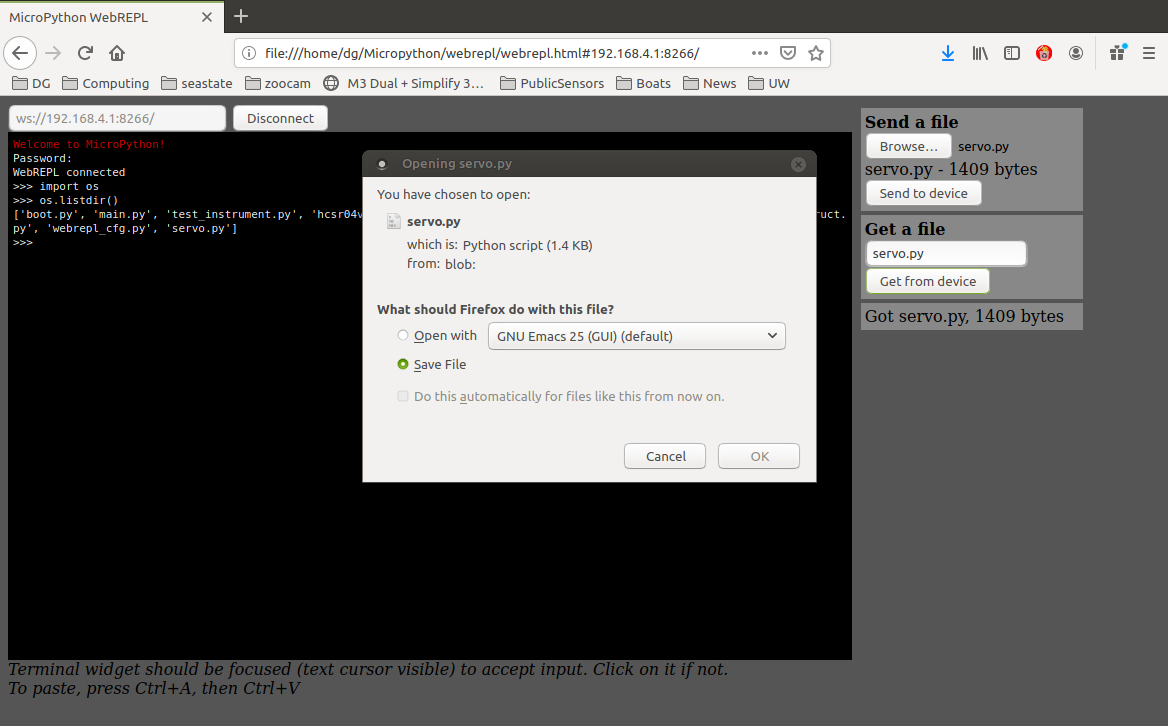
\includegraphics[width=5cm]{Images/WebREPLdownload.png}
%		\caption[A WebREPL session with download.]{An active WebREPL session, showing the commands to list the files on the microcontroller (main terminal frame), a file download (right side panel, and a prompt for how to save or open the file.}
%		\labfig{WebREPL_download}
%	\end{center}
%\end{marginfigure}
%\textbf{To download a file from your microcontroller (\reffig{WebREPL_download}):}
%\begin{enumerate}
%	\item Enter the name of the file in the textbox under the \texttt{Get a file} prompt.
%	
%	You can see which files are on the microcontroller with the \Micropython commands:
%	\begin{lstlisting}[language=Python]
%	import os
%	os.listdir()
%	\end{lstlisting}
%	
%	\item Click the \texttt{Get from device} button. 
%	\item \texttt{WebREPL} will download the file, report its name and size in the text box, and prompt you to save or open the file on your laptop.
%\end{enumerate}
%
%
%%\subsubsection{WiFi connections via \texttt{Secure Shell} in Chrome}
%%When your microcontroller is not connected by a USB cable to your laptop, you will connect to it over WiFi.
%%If \mpfshell is installed on your  machine, it is likely the best option to connect to your microcontroller over WiFi (see the \htmladdnormallink{mpfshell github site}{https://gist.github.com/hardye/657385210c5d613e69cb5ba95e8c57a7} for instructions on how to connect to a microcontroller via WiFi).
%%\texttt{WebREPL} is also a good alternative, but for \texttt{WebREPL} to work it must be enabled on your microcontroller.
%%If it is not enabled, and if you prefer a browser-based communication method, you can use an alternative like \htmladdnormallink{Secure Shell}{https://chrome.google.com/webstore/detail/secure-shell/pnhechapfaindjhompbnflcldabbghjo?hl=en} instead. 
%%
%%(including logging onto your microcontroller to enable WebREPL).
%%
%%in some ways nicer to use than Secure Shell 
%%
%%For this you will need a different app than you used for serial communication – you will need a terminal interface through which you can remotely log onto your microcontroller, to issue commands and obtain sensor readings. 
%% is an app that provides this capability.
%%
%%
%%
%%In many cases you will be able to use WebREPL instead of Secure Shell -- it also enables you to log onto your microcontroller. 
%%
%
%\subsection{WiFi connections using \mpfshell}
%\mpfshell is as useful for connecting to your ESP8266 remotely over WiFi as it is for connecting directly via USB. 
%To connect with your microcontroller using \mpfshell over WiFi:
%\begin{enumerate}
%	\item Make sure \texttt{webrepl} is enabled (see instructions above for WebREPL if you're not sure).
%	\item In a terminal window, launch \mpfshell:
%	\begin{lstlisting}[language=Python]
%	mpfshell
%	\end{lstlisting}
%	\item Open the connection over WiFi with	
%	\begin{lstlisting}[language=Python]
%	open ws:192.168.4.1
%	\end{lstlisting}
%	
%	In this command, the number \texttt{192.168.4.1} is the microcontroller's IP number. 
%	If the microcontroller's AP is activated and your laptop is connected to it, the default number is correct.
%	
%	If you are connecting via a router, then you need to replace this number with the IP assigned to your microcontroller (see the \texttt{wlan.ifconfig()} command in the instructions for WebREPL).
%	
%	\item At the prompt, enter your \texttt{webrepl} password.
%	
%	You should then see the \verb|mpfs [/]>| prompt showing that you have successfully connected through \mpfshell.
%\end{enumerate}
%
%%With \texttt{webrepl} activated on your microcontroller (as described above) and AP mode activated, connect from \mpfshell using
%%If you are connected via a router, you will need to modify this command to correspond to the IP number assigned by the router to your microcontroller. 
%%You will be prompted to enter your \texttt{webrepl} password, after which you will be connected and a
%All the \mpfshell file transfer and REPL capabilities work the same over WiFi as when connected via USB.
%
%\loadMilestone{mlst:01b} % load milestone with tags id: mlst:01b
%
%%\todo{Recreate images for BeagleTerm, WebREPL and Secure Shell descriptions.}
%%\todo{Need to include specific sections about how to do REPL, copy/pasting and file transfer.}
%\todo{Include code to disable debug output, i.e., 
%	
%	import esp
%	
%	esp.osdebug(None)}
